% Section V: Experimental setup and evaluation protocol (target 0.90 pages with the layout figure).
% Sources: docs/data_rules.md "Evaluation", docs/decisions.md t3-g (and addenda), configs/eval_layouts.yaml,
% data/eval/eval_sheet.csv. Results: Section VI.
\section{Experimental Setup and Evaluation Protocol}
\label{sec:experiments}

\subsection{Evaluated Policy and Source Layouts}
\label{sec:layouts}
The evaluation tests one policy: ACT trained on \emph{all} at its final checkpoint
(Section~\ref{sec:execution}), from a single training run. No comparison
condition is evaluated; the study measures whether the complete application
performs the packing task and how it fails.

The items are placed in five predefined source layouts
(Fig.~\ref{fig:layouts}). Each layout fixes the grasp point of every item in
the robot base frame, inside the region where items were grasped in the
three-item demonstrations (457--747~mm from the base axis), with the items at
least 21~cm apart and oriented as in the demonstrations. The layouts vary
which item lies nearest the robot: the carrot in two, the Oreo in one, and the
RITZ in two. In three layouts the RITZ lies nearer than the Oreo, so that
picking the nearest item first would break the packing order. The containers
stay where they were during data collection.

The table carries no marks. Instead, a top-camera photograph was saved for
each layout once its items were in place (Fig.~\ref{fig:layouts}). Before each trial, the execution
program shows the live top image with this photograph blended in and a circle
at each grasp point, located by an affine map from the base frame to the image
fitted to ten demonstrated grasps (rms error 18~px, about 2~cm on the table).
The operator places the items to match the photograph.

\begin{figure*}[t]
\centering
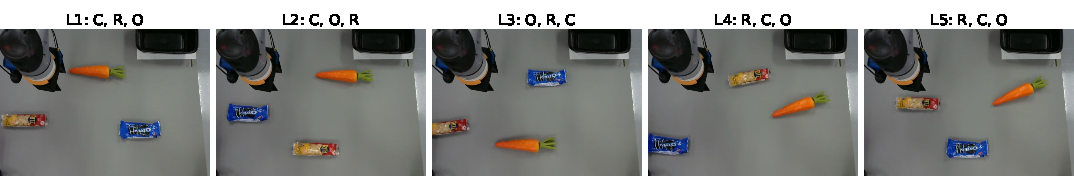
\includegraphics[width=\textwidth]{figures/fig_layouts.pdf}
\caption{The five source layouts, seen by the top camera in the photographs
used to place the items. Each label lists the items from nearest to farthest
from the robot base axis (C carrot, O Oreo, R RITZ). The gripper at the ready
pose is at the upper left and the black box at the upper right; the meal box
lies outside the view.}
\label{fig:layouts}
\end{figure*}
% Made by paper/figures/make_fig_layouts.py from data/eval/layouts/L*.jpg. Grasp points (x, y) in the base
% frame, mm (configs/eval_layouts.yaml): L1 C(80,-450) O(250,-690) R(-200,-600); L2 C(200,-480) O(-180,-580)
% R(100,-740); L3 C(30,-700) O(150,-460) R(-220,-640); L4 C(280,-620) O(-200,-680) R(60,-470);
% L5 C(250,-560) O(80,-720) R(-60,-560).

\subsection{Trial Procedure}
\label{sec:trials}
Each layout is tested four times, giving 20 trials in one session. Every round
visits all five layouts, and each round starts one layout later than the
previous one (L1--L5, then L2--L5 and L1, and so on), so that no layout is
always early or late in the session. Each trial is a separate run of the
execution program. The robot moves to the ready pose with the gripper open,
the operator places the items, and a single start key begins autonomous
execution. The operator then touches neither the items nor the robot. The trial
ends when all items have been released and the gripper has lifted, at the
180-s limit of Section~\ref{sec:execution}, or when the operator intervenes,
which counts as a failure. The controller settings are those of
Section~\ref{sec:limits}: collision detection at a 30\% threshold and a tool
mass of 0~kg.
Each trial leaves its own log of robot states, targets, gripper commands, and
inference times, together with a video of the three camera views whose frame
times are stored on the clock of the log.

\subsection{Success Criteria and Measures}
\label{sec:measures}
A trial is a \emph{complete success} when, within 180~s and without
intervention, the carrot rests in the black box, the Oreo in the large hole,
and the RITZ in the small hole, with the gripper open. The snacks are longer
than their holes, so a snack counts as placed when it rests touching the inside
of its hole, tilted or not; a snack on the rim does not. The criterion,
fixed before the trials, concerns the final state and does not require the
packing order, which is reported separately.

Each item is judged in four stages from the trial video: \emph{grasp} (lifted
off the table, including re-grasps within the limit), \emph{transport} (carried
above a container without dropping), \emph{place} (released and resting inside
some container), and \emph{correct} (that container is the assigned one). An
item that never reached a stage, such as the items left after the policy
stalled on an earlier one, is counted as not attempted there rather than as
failed. Each stage's rate is thus conditional on reaching the stage, which
locates the weak stage, while the share of the 60 items placed correctly shows
how early failures cascade. Borderline final states were decided by the
operator, who watched every trial.

The primary measures are the complete successes out of 20 with a Wilson 95\%
confidence interval~\cite{wilson1927probable}, the stage rates, the correctly
placed items out of 60, and the completion time of the successful trials, from
the start key to the last release. Failed trials are assigned a main cause and
excluded from the time statistics, so that fast failures do not appear
advantageous. Grasping is described by the share of items grasped at the first
close, the share of all gripper closes that lifted an item, and the recovery
rate: items grasped after at least one miss on them, over items with a miss.
An order error is recorded when an item is picked up and carried before an item
that precedes it in the packing order; releases into a wrong compartment are
counted separately. As a reference, the three-item demonstrations lasted
58.8~s on average (Table~\ref{tab:datasets}), measured from the start to the end
of recording rather than to the last release. Supporting measures are the
inference time, computed once per prediction, the servo interval, and the
number of late cycles and holds.
% TODO: add wilson1927probable (E. B. Wilson, J. Amer. Statist. Assoc., 1927) to references.bib.
